% !TeX TS-program = xelatex
\documentclass[aspectratio=169, 12pt, xcolor=table]{beamer}
\usefonttheme{professionalfonts}
\usefonttheme{serif}
\usepackage[T1]{fontenc}
\usepackage{fontspec-xetex}

\usepackage{tikz}

\usepackage{adjustbox}
\usepackage{booktabs}
\usepackage{ifthen}
\usepackage{listings}
\usepackage{subcaption}

\usetikzlibrary{shapes.geometric, arrows}

\setmainfont{Lato}

%\PassOptionsToPackage[more=table]{xcolor}

% Local configuration
\renewcommand{\figurename}{}
\DeclareCaptionFormat{custom}
{%
	\tiny #3
}
\captionsetup{format=custom}

% Title stuff
\title{Games Technologies}
\subtitle{Object-Oriented Programming}
\date{Week 02}
\author{Vassilis Markos, Mediterranean College}

\usetheme{streamline}

% Local Commands
\newcommand{\ohref}[1]{\href{#1}{\texttt{#1}}}
\newcommand{\listindex}[2]{{\underset{#1}{\small #2}}}

% Code listings

\definecolor{codegreen}{rgb}{0,0.6,0}
\definecolor{codegray}{rgb}{0.5,0.5,0.5}
\definecolor{codepurple}{rgb}{0.58,0,0.82}
\definecolor{backcolour}{rgb}{0.95,0.95,0.92}

\lstdefinestyle{mystyle}{
	backgroundcolor=\color{backcolour},   
	commentstyle=\color{codegreen},
	keywordstyle=\color{magenta},
	numberstyle=\tiny\color{codegray},
	stringstyle=\color{codepurple},
	basicstyle=\ttfamily\footnotesize,
	breakatwhitespace=false,         
	breaklines=true,                 
	captionpos=b,                    
	keepspaces=true,                 
	numbers=left,                    
	numbersep=5pt,                  
	showspaces=false,                
	showstringspaces=false,
	showtabs=false,                  
	tabsize=2
}

\lstset{style=mystyle}

% Tikz style

\tikzstyle{startstop} = [ellipse, rounded corners, minimum width=2cm, minimum height=0.8cm, text centered, draw=black, fill=none]
\tikzstyle{io} = [trapezium, trapezium left angle=70, trapezium right angle=110, minimum width=2cm, minimum height=0.8cm, text centered, draw=black, fill=none]
\tikzstyle{process} = [rectangle, minimum width=2cm, minimum height=0.8cm, text centered, draw=black, fill=none]
\tikzstyle{decision} = [diamond, minimum width=2cm, minimum height=0.8cm, text centered, draw=black, fill=none]
\tikzstyle{arrow} = [thick,->,>=stealth]

\tikzstyle{simple node} = [rectangle, draw=black, minimum width = 0.8cm, minimum height = 0.6cm]

% makeatletter stuff

\makeatletter
\newcommand{\arabicthree}[1]{\expandafter\@arabicthree\csname c@#1\endcsname}
\newcommand{\@arabicthree}[1]{\ifnum #1<100 0\fi\ifnum #1<10 0\fi\number#1}
\makeatother

\newcounter{exno}
\setcounter{exno}{0}

\newcommand{\exno}{\stepcounter{exno}In--class Exercise \#\arabicthree{exno}}

\begin{document}
	
	\begin{frame}
		\titlepage
	\end{frame}
	
	\begin{frame}{Contents}
		\tableofcontents
	\end{frame}
	
	\section{Object-Oriented Programming}\label{sec:key-cshar-constructs}
	
	\sectionframe
	
	\begin{frame}{Programmer Humour}
		\begin{figure}
			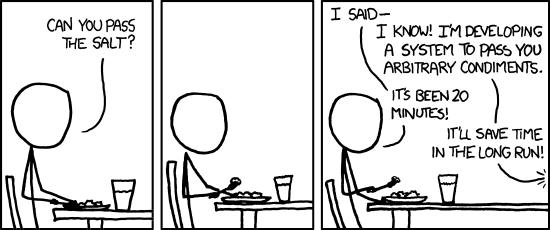
\includegraphics[width=0.75\textwidth]{assets/the_general_problem.png}
			\caption{Source: \href{https://xkcd.com/974/}{https://xkcd.com/974/}.}
		\end{figure}
	\end{frame}

	\begin{frame}{What is Object-Oriented Programming?}
		By Wkipedia's \href{https://en.wikipedia.org/wiki/Object-oriented_programming}{definition}:
		\begin{quote}
			Object-oriented programming (OOP) is a programming paradigm based on objects -- software entities that encapsulate data and function(s).
		\end{quote}
		So, essentially, we bind data together with actions frequently performed on / with those data.
	\end{frame}

	\begin{frame}{Why Object-Oriented Programming}
		\begin{itemize}[<+->]
			\item There are many reasons to use Object-Oriented Programming (OOP)
		\end{itemize}
	\end{frame}

	\begin{frame}{Why NOT OOP?}
		OOP is not a one-size-fits-all solution
		\begin{itemize}[<+->]
			\item 
		\end{itemize}
	\end{frame}
	
	\section{Fun Time!}\label{sec:fun-time}
	
	\sectionframe
	
	\setcounter{exno}{0}
	
	\begin{frame}[fragile]{\exno}
		Make all transcriptions from Python to C\# found in:
		\begin{center}
			\texttt{lab/transcriptions.pdf}
		\end{center}
		Use any only resources you might find useful.
	\end{frame}
	
	\begin{frame}{Homework}
		Complete any incomplete lab exercises and then proceed to complete any missing parts of the game lab discussed in class today.
	\end{frame}
	
	\begin{frame}{Any Questions?}
		\begin{minipage}{0.35\textwidth}
			\raggedright
			Do not forget to fill in the questionnaire shown right!
		\end{minipage}\hfill
		\begin{minipage}{0.58\textwidth}
			\vspace{0pt}
			\raggedleft
			
\includegraphics[scale=0.4]{../../assets/post_lesson_assessment.png}
			\centering
			\ohref{https://forms.gle/dKSrmE1VRVWqxBGZA}
		\end{minipage}
	\end{frame}
	
\end{document}